\documentclass[../main-report.tex]{subfiles}
\begin{document}

\section{Giới thiệu hệ thống}
Khóa luận hướng đến việc áp dụng công nghệ \gls{blockchain} để giải quyết các vấn đề về tính minh bạch, công khai và tin cậy của ứng dụng gây quỹ cộng đồng theo mô hình truyền thống đã đề cập ở mục \ref{sec:problem}, \ref{sec:related-work}. Nhóm tác giả sử dụng \gls{blockchain} cho việc lưu trữ các thông tin về tài chính, các giao dịch của người dùng trong hệ thống nhằm hạn chế việc lưu các thông tin này trên bất kì một bên thứ ba nào. Hơn thế nữa, hệ thống sử dụng hợp đồng thông minh cho các lệnh liên quan tài chính trong hệ thống. Các lệnh này được thực hiện một cách tự động và chính xác, tránh sự can thiệp hay tác động từ yếu tố con người vào hệ thống. Với hợp đồng thông minh, nhóm tác giả cũng bổ sung các tính năng như tự động hoàn tiền khi mục tiêu gây quỹ chiến dịch không thành công; bỏ phiếu để giải ngân, tăng quyền hạn cho người đóng góp chiến dịch.

Bên cạnh đó, hệ thống của nhóm tác giả cũng sử dụng một phần dữ liệu được lưu trữ tập trung nhằm cải thiện tốc độ đọc ghi với các dữ liệu không cần độ tin cậy cao.

\section{Quy trình gây quỹ cộng đồng}
Đây là quy trình gây quỹ cộng đồng trong hệ thống của nhóm tác giả.
\subsection{Các đối tượng trong quy trình}
Trong quy trình gây quỹ, có các đối tượng sau:
\begin{itemize}
\item \textbf{Người tạo chiến dịch:} là những cá nhân / tổ chức có nhu cầu gây quỹ vì mục đích từ thiện, hướng tới cộng đồng.
\item \textbf{Hệ thống:} là hệ thống gây quỹ trung gian, đứng giữa người tạo chiến dịch và người đóng góp.
\item \textbf{Người đóng góp:} là người ủng hộ đóng góp tiền cho chiến dịch gây quỹ.
\end{itemize}

\subsection{Sơ đồ quy trình gây quỹ}
Sơ đồ quy trình gây quỹ được thể hiện ở hình \ref{fig:crowdfunding-proccess}.

\begin{figure}[ht!]
\begin{center}
\label{fig:crowdfunding-proccess}
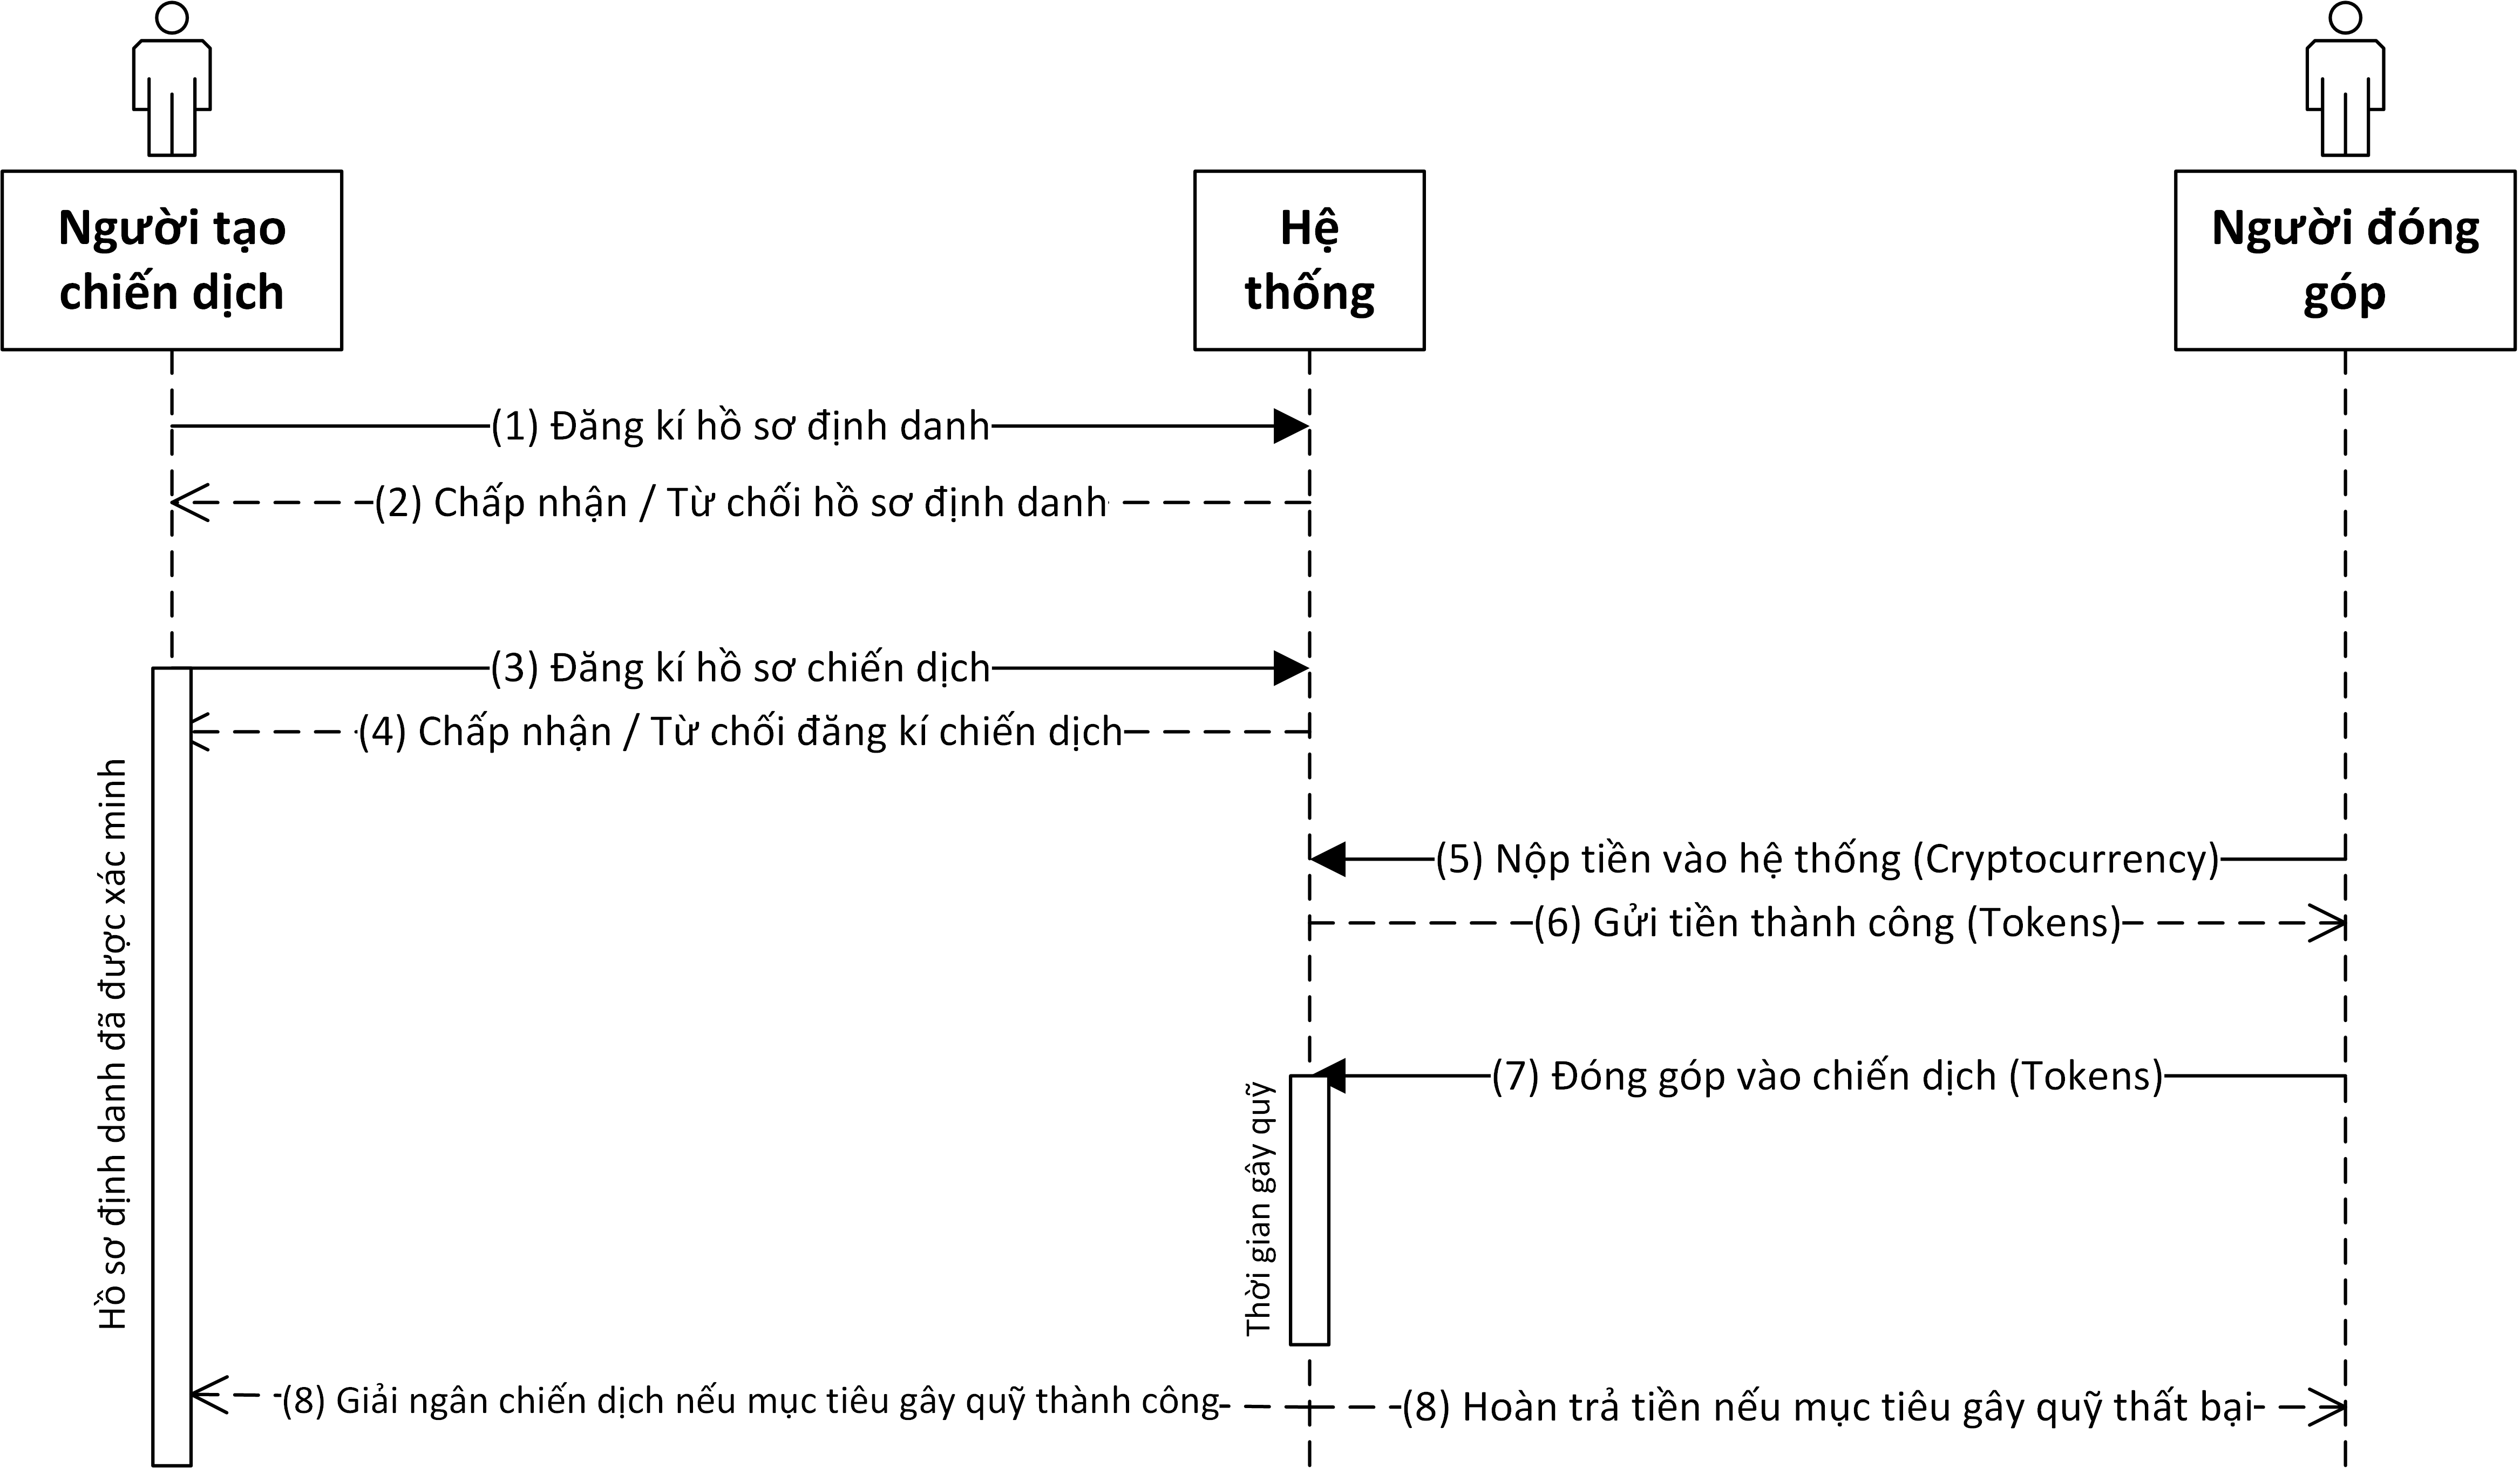
\includegraphics[scale=0.75]{crowdfunding-process}
\caption{Sơ đồ quy trình gây quỹ cộng đồng}
\end{center}
\end{figure}

Quy trình này được diễn giải như sau:

\begin{enumerate}[label=(\arabic*)]
\item Người tạo chiến dịch sẽ tiến hành tạo lập hồ sơ định danh bao gồm thông tin cá nhân cơ bản và thông tin chứng minh định danh.
\item Hệ thống (nhân viên xác minh) tiến hành xác minh hồ sơ định danh và chấp nhận hay từ chối hồ sơ. Nếu hồ sơ định danh được chấp nhận thì hồ sơ đó được phép gọi lệnh tạo chiến dịch, ngược lại thì không.
\item Người tạo chiến dịch tiếp tục tạo lập hồ sơ chiến dịch gây quỹ nếu hồ sơ định danh được chấp nhận.
\item Hệ thống (nhân viên xác minh) tiến hành xác minh hồ sơ chiến dịch và chấp nhận hay từ chối hồ sơ. Hồ sơ được chấp nhận sẽ được công khai lên hệ thống và cho phép người đóng góp ủng hộ tiền. Ngược lại thì không.
\item Người đóng góp muốn ủng hộ tiền cho một chiến dịch thì cần sử dụng \gls{cryptocurrency} (\glsdesc{cryptocurrency}) gửi vào hệ thống (lúc này là hợp đồng thông minh) để sử dụng các chức năng trong hệ thống.
\item Sau khi người đóng góp gửi tiền vào hệ thống, hệ thống sẽ lưu số tiền người gửi vào dưới dạng một giá trị được gọi là token. Người đóng góp sử dụng token này trong các giao dịch nội bộ của hệ thống. Token này có thể được đổi ngược lại sang đồng \gls{cryptocurrency} với giá tương ứng
\item Người đóng góp ủng hộ tiền cho một chiến dịch (chiến dịch đã được xác minh) bằng một lượng token mà người đóng góp mong muốn và đang có.
\item Mỗi chiến dịch sẽ có một khoảng thời gian để kêu gọi đóng góp, và một mục tiêu là số lượng token cần đạt được. Khi hết thời gian kêu gọi đóng góp, nếu chiến dịch hoàn thành mục tiêu thì sẽ tiến hành cho người tạo chiến dịch giải ngân. Ngược lại, lượng token đã đóng góp sẽ được hoàn lại cho người đóng góp.
\end{enumerate}
\section{Kiến trúc hệ thống}
Kiến trúc hệ thống được thể hiện ở hình \ref{fig:system-architecture}.

\begin{figure}[ht!]
\begin{center}
\label{fig:system-architecture}
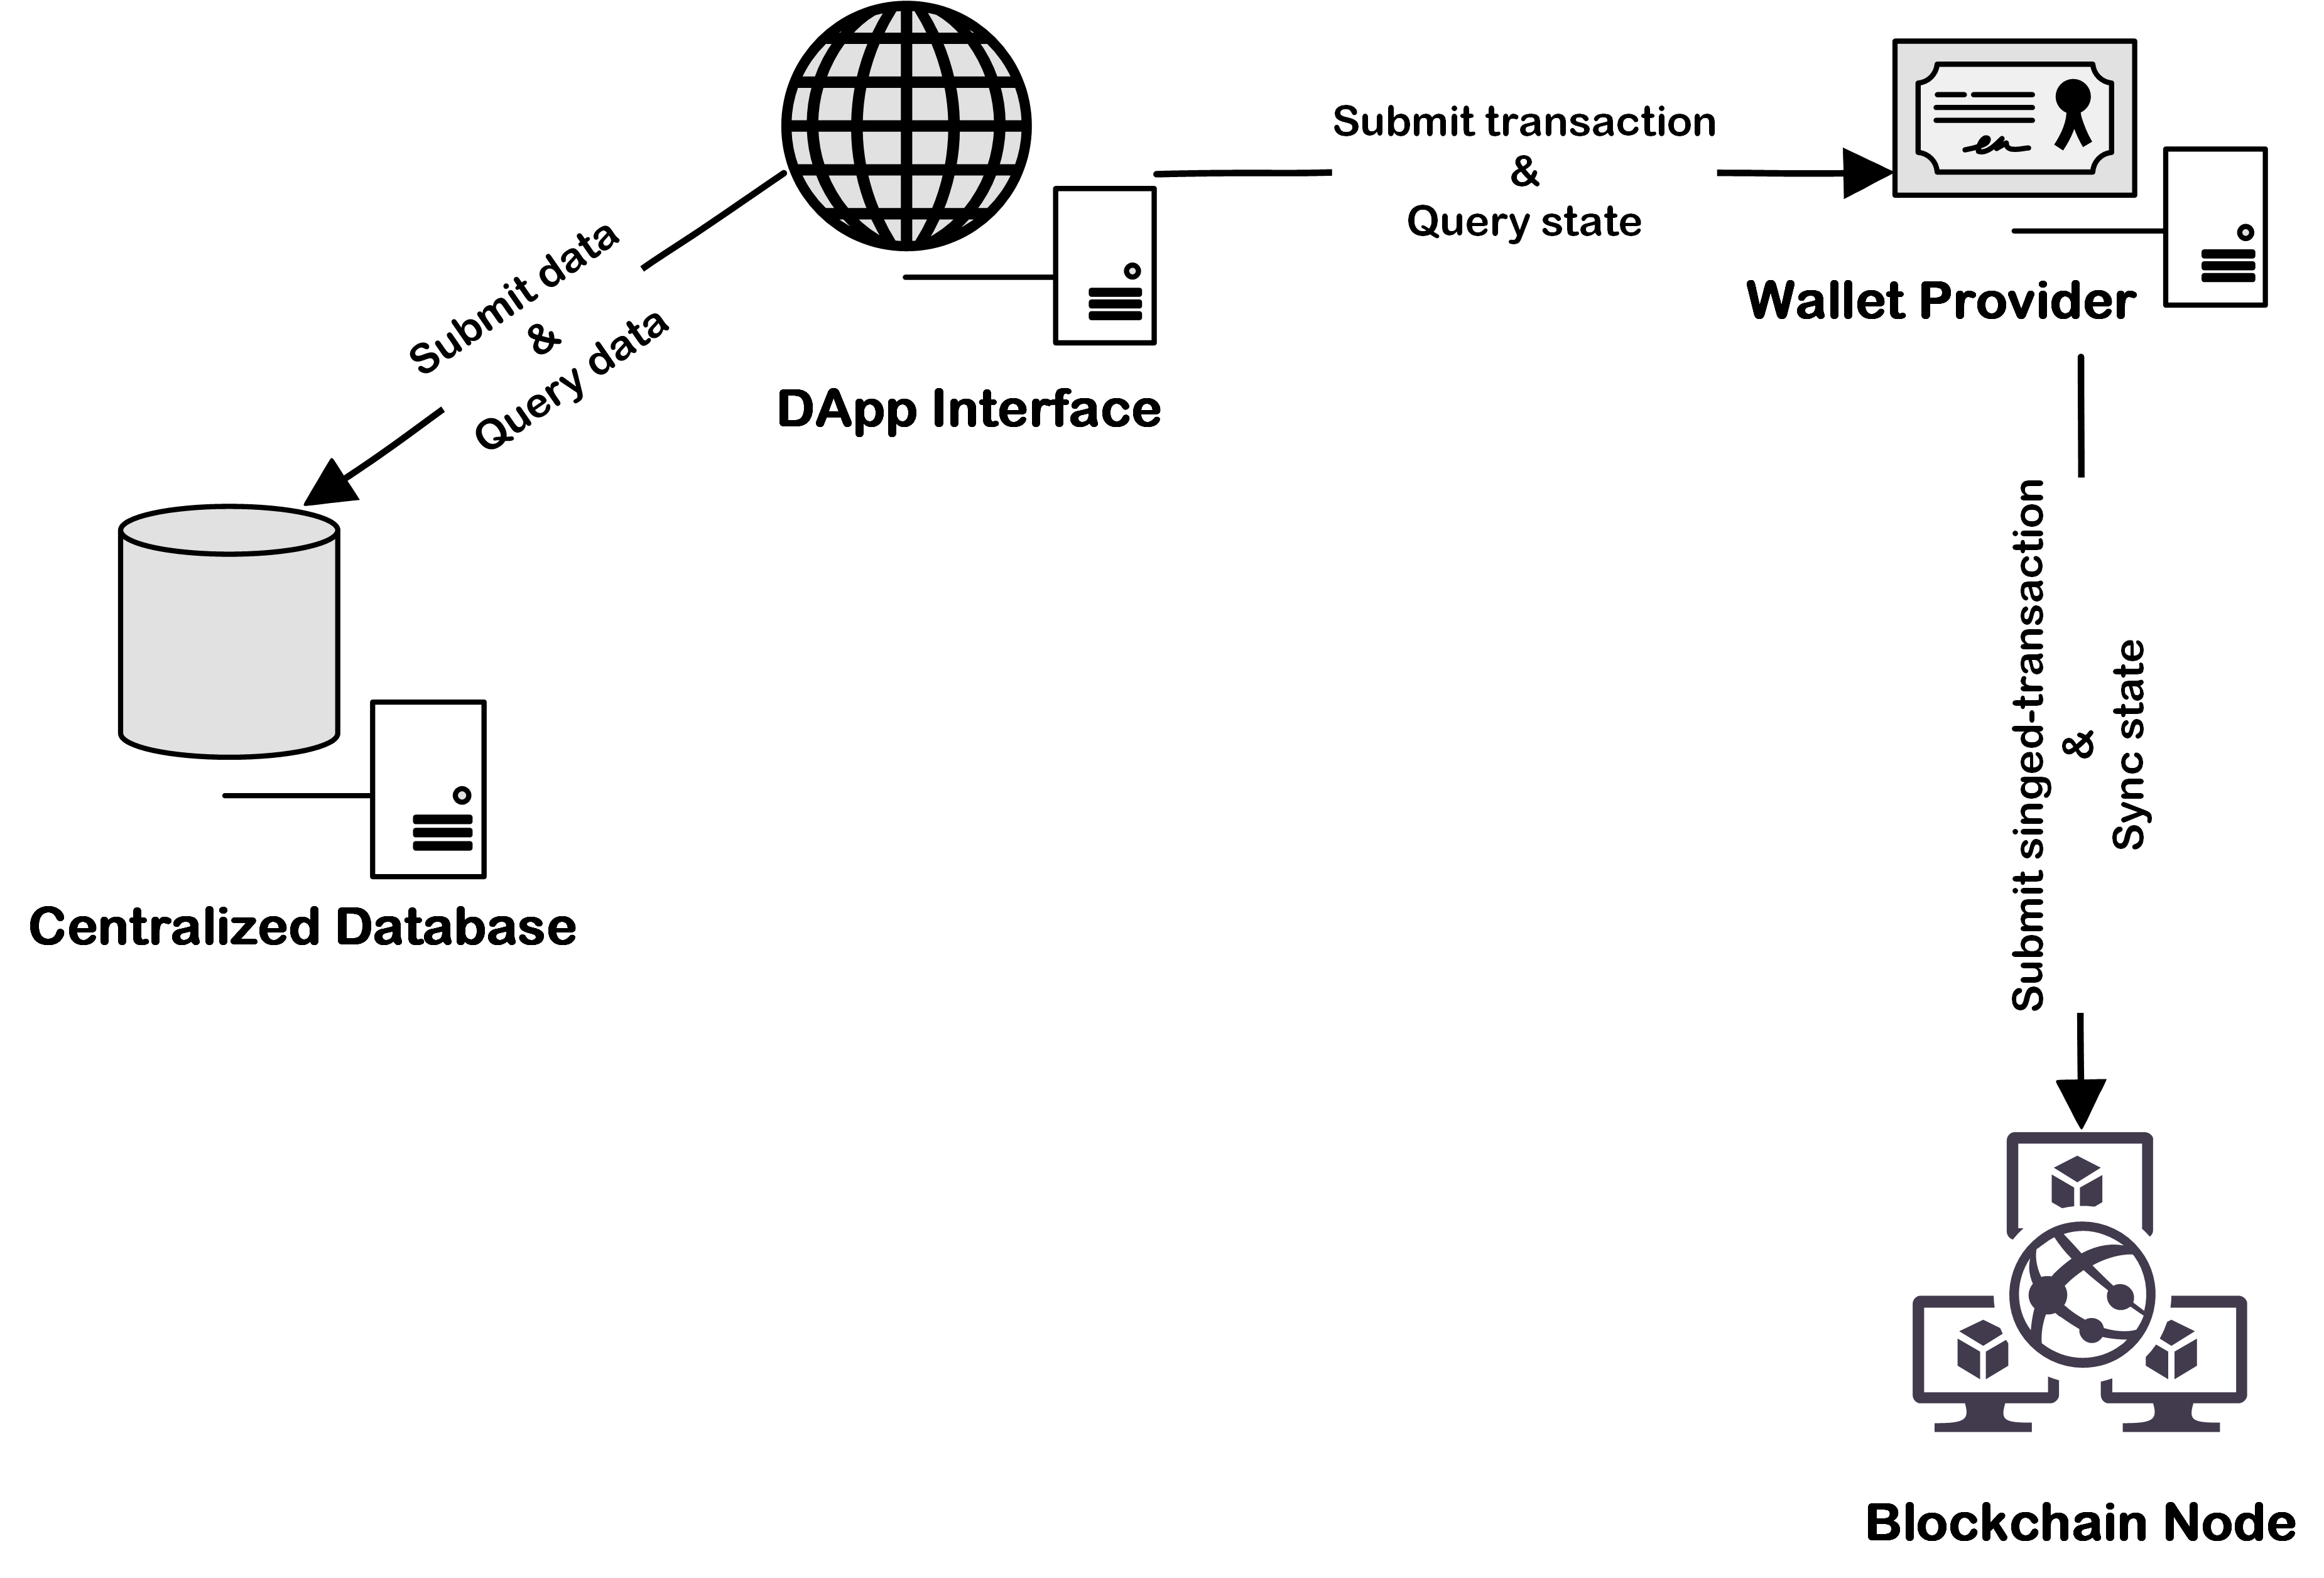
\includegraphics[scale=0.9]{system-architecture}
\caption{Sơ đồ kiến trúc hệ thống}
\end{center}
\end{figure}

Các thành phần và vai trò của từng thành phần trong hệ thống mà nhóm tác giả đề xuất như sau:

\begin{itemize}
\item \textbf{DApp Interface} - là một giao diện ứng dụng phi tập trung, nơi người dùng sẽ tương tác trực tiếp. \textit{DApp Interface} sẽ tạo ra các \gls{transaction} để gọi các hàm có trong hợp đồng thông minh và chuyển các \gls{transaction} này tới Wallet Provider thực hiện công đoạn tiếp theo. Và đây cũng là nơi tương tác với cơ sở dữ liệu tập trung trong mô hình. Thực chất \textit{DApp Interface} chỉ là một giao diện front-end tĩnh chạy ở phía người dùng.
\item \textbf{Wallet Provider} - là ứng dụng phi tập trung có nhiệm vụ xác nhận và kí transaction (\textit{sign transaction}) do \textit{DApp Interfac}e gửi tới trong mô hình, sau đó thực hiện gửi các \gls{transaction} đã được kí (\textit{signed-transaction}) đến mạng lưới \gls{blockchain}. Wallet cũng làm nhiệm vụ lưu trữ thông tin về khóa bí mật của người dùng.
\item \textbf{Blokchain Node} - là một nút trong mạng \gls{blockchain} mà \textit{Wallet Provider} tương tác để lưu trữ các dữ liệu phi tập trung, các dữ liệu phi tập trung trong trường hợp này là các mã hợp đồng thông tin và các giá trị trong hợp đồng.
\item \textbf{Centralized Database} - là một cơ sở dữ liệu tập trung, được dùng để lưu trữ một số thông tin như mô tả chiến dịch.
\end{itemize}

\section{Các chức năng}
\subsection{Tổng quan các chức năng}
Tổng quan các chức năng trong hệ thống được thể hiện ở hình \ref{fig:usecase-diagram}. Với sơ đồ được thể hiện có các đối tượng sau:

\begin{itemize}
\item \textbf{Creator} - là người tạo chiến dịch gây quỹ.
\item \textbf{Donor} - là người đóng góp, ủng hộ tiến cho chiến dịch gây quỹ.
\item \textbf{Verifier} - là người xác minh cho hồ sơ định danh và hồ sơ gây quỹ, là nhân viên trong hệ thống hoặc tình nguyện viên của hệ thống.
\item \textbf{Deployer} - là người vận hành hệ thống hay người triển khai các hợp đồng thông minh.
\end{itemize}

\begin{figure}[ht!]
\begin{center}
\label{fig:usecase-diagram}
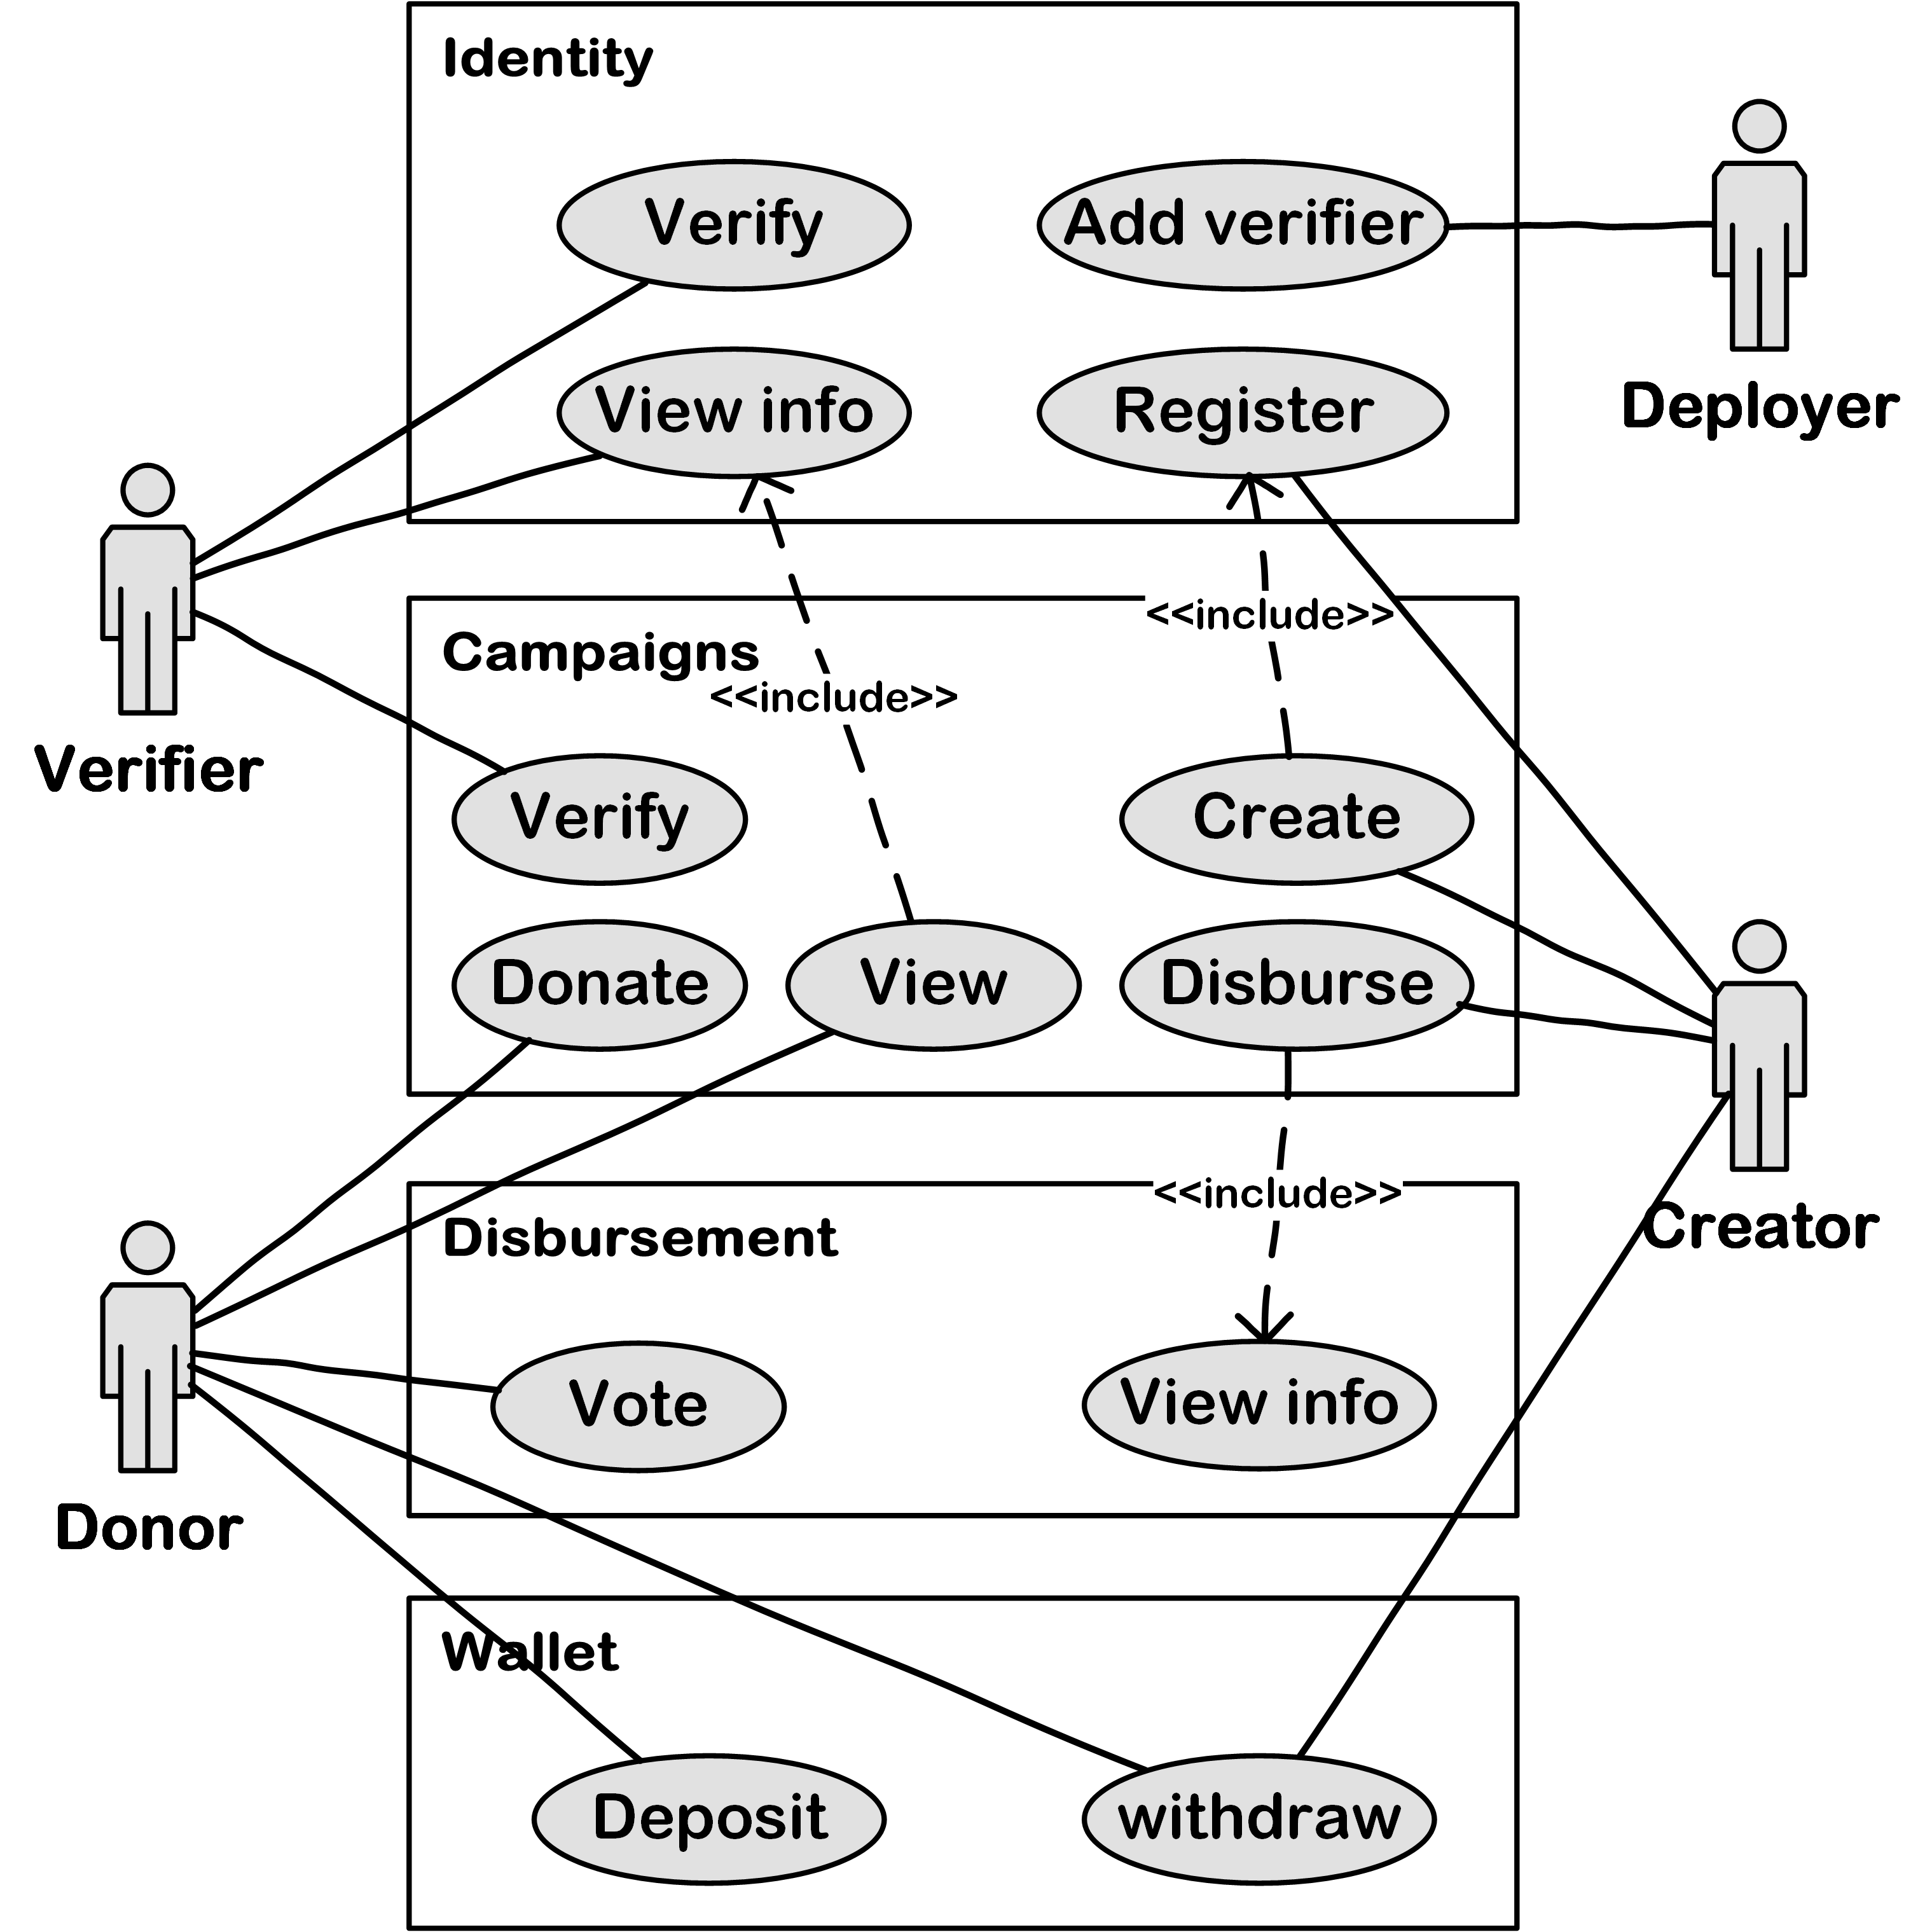
\includegraphics[scale=1]{usecase}
\caption{Sơ đồ tổng quan các chức năng trong hệ thống}
\end{center}
\end{figure}

Các chức năng trong hệ thống được phân nhóm thành các cụm theo 4 hệ thống con tương ứng các hợp đồng thông minh, cụ thể:

\begin{itemize}
\item \textbf{Wallet:}
\begin{itemize}
\item \textit{Deposit} - cho phép người dùng gửi tiền vào hệ thống, đổi lấy giá trị giao dịch nội bộ trong hệ thống.
\item \textit{Withdraw} - cho phép người dùng chuyển đổi từ giá trị giao dịch nội bộ trong hệ thống thành đồng tiền mã hóa bên ngoài.
\end{itemize}
\item \textbf{Campaigns:}
\begin{itemize}
\item \textit{Create} - tạo lập hồ sơ chiến dịch gây quỹ.
\item \textit{Verify} - xác minh chấp nhận / từ chối một hồ sơ gây quỹ.
\item \textit{View} - xem thông tin chiến dịch.
\item \textit{Donate} - cho phép người đóng góp ủng hộ tiền cho một chiến dịch, đóng góp dưới dạng giá trị trao đổi trong hệ thống.
\item \textit{Disburse} - cho phép người tạo lập chiến dịch tiến dịch lệnh gọi giải ngân cho chiến dịch.
\end{itemize}
\item \textbf{Identity:}
\begin{itemize}
\item \textit{Add verifier} - thêm các verifier vào danh sách.
\item \textit{Register} - cho phép người tạo chiến dịch gây quỹ tiến hành đăng kí hồ sơ định danh.
\item \textit{Verify} - cho phép verifier tiến hành xác mịnh chấp nhận / từ chối một hồ sơ định danh.
\item \textit{View info} - xem thông tin hồ sơ định danh (các thông tin công khai). 
\end{itemize}
\item \textbf{Disbursement:}
\begin{itemize}
\item \textit{Vote} - cho phép người đóng góp bỏ phiếu chấp nhận giải ngân cho một chiến dịch.
\item \textit{View info} - trả về thông tin xác nhận giải ngân (chiến dịch có thỏa điều kiện hay chưa), phục vụ cho chức năng giải ngân trong chiến dịch gây quỹ.
\end{itemize}
\end{itemize}
\subsection{Chức năng nộp tiền và rút tiền}
\subsubsection{Mục tiêu}

\subsubsection{Sơ đồ hoạt động}

\subsection{Chức năng quản lý định danh}
\subsubsection{Mục tiêu}
Do trong \gls{blockchain} mỗi người dùng sẽ được xác định bởi các \gls{address} (địa chỉ), các địa chỉ này hoàn toàn tách biệt với danh tính của người dùng, tức nó không bao gồm danh tính hay bất cứ thông tin nào như địa chỉ IP, định vị, \ldots. Do đó có thể nói mỗi người dùng trên mạng \gls{blockchain} là ẩn danh \cite{henry2018blockchain}. Để tăng tính tin cậy cho chiến dịch gây quỹ thì cần thiết phải gắn mỗi địa chỉ người dùng cho một hồ sơ định danh, vì vậy một địa chỉ người dùng muốn đăng kí tạo chiến dịch thì bắt buộc địa chỉ đó đã có hồ sơ định danh và hồ sơ định danh đó phải được xác minh. Việc tạo lập hồ sơ định danh chỉ bắt buộc với địa chỉ người dùng nào muốn tạo chiến dịch, còn đối với người đóng góp vào chiến dịch thì không bắt buộc.

Hồ sơ định danh có 2 loại thông tin cơ bản là: 

\begin{itemize}
\item \textbf{Thông tin công khai:} là những thông tin cơ bản của người tạo chiến dịch như họ tên, địa chỉ, ngày sinh. Việc công khai thông tin là bắt buộc đối với người tạo chiến dịch.
\item \textbf{Thông tin cá nhân nhạy cảm}: là các thông tin cá nhân bí mật, được dùng để chứng minh cho các thông tin được công khai. Do đó cần lưu trữ thông tin cá nhân nhạy cảm một cách bí mật và toàn vẹn.
\end{itemize}

Yêu cầu về chia sẻ thông tin cá nhân giữa người dùng và người xác minh phải đảm bảo được các yếu tố:

\begin{enumerate}
\item Chỉ có người dùng và người xác minh mới có thể đọc được thông tin.
\item Việc xác minh cho một hồ sơ được minh bạch. Tức biết ai là người đã xác minh cho hồ sơ, và vào thời gian nào.
\end{enumerate}

\subsubsection{Cách hoạt động}
Nhóm tác giả chia làm 2 tiến trình hoạt động cho chức năng này:

\begin{itemize}
\item Tạo lập và lưu trữ hồ sơ định danh.
\item Chia sẻ thông tin hồ sơ định danh.
\end{itemize}

Các đối tượng trong chức năng định danh bao gồm:

\begin{itemize}
\item \textbf{Người tạo lập hồ sơ (người dùng - user):} là người tạo hồ sơ định danh, hay người tạo chiến dịch gây quỹ.
\item \textbf{Người xác minh hồ sơ (verifier)}: người xác minh cho một hồ sơ định danh. Có thể là nhân viên trong hệ thống, tình nguyện viên.
\item \textbf{Người vận hành hệ thống (deployer):} người quản lí danh sách các verifier. Hay người sẽ triển khai hợp đồng thông minh lên \gls{blockchain}.
\end{itemize}

Cách thức tạo lập và lưu trữ hồ sơ định danh được thể hiện ở hình \ref{fig:identity-process-1}. Cụ thể:

\begin{itemize}
\item Người tạo lập hồ sơ định danh tiến hành nhập thông tin định danh.
\item Người tạo lập hồ sơ nhập một chìa khóa bảo vệ hồ sơ định danh, được gọi là \textbf{SecretKey}. SecretKey được dùng cho 2 mục đích:
\begin{enumerate}[label=(\roman*)]
\item Làm khóa (key) cho thuật toán AES dùng để mã hóa các thông tin nhạy cảm của người dùng trước khi lưu trữ.
\item SecretKey sẽ được mã hóa bằng thuật toán RSA bởi khóa công khai của verifier, sau đó chuỗi mã hóa sẽ được lưu trữ trên \gls{blockchain}.
\end{enumerate}
\item Người tạo lập chọn khóa công khai của verifier (chọn một verifier trong danh sách các verifier), khóa này được dùng để mã hóa SecretKey của người tạo lập hồ sơ.
\item Thông tin công khai và khóa bí mật đã mã hóa sẽ được lưu trữ trên hợp đồng thông minh trong blockchain. Thông tin bí mật đã mã hóa sẽ được lưu trữ trên một mạng lưu trữ phi tập trung (ở đây nhóm tác giả đề xuất \acrshort{ipfs}).
\end{itemize}

\begin{figure}[ht!]
\begin{center}
\label{fig:identity-process-1}
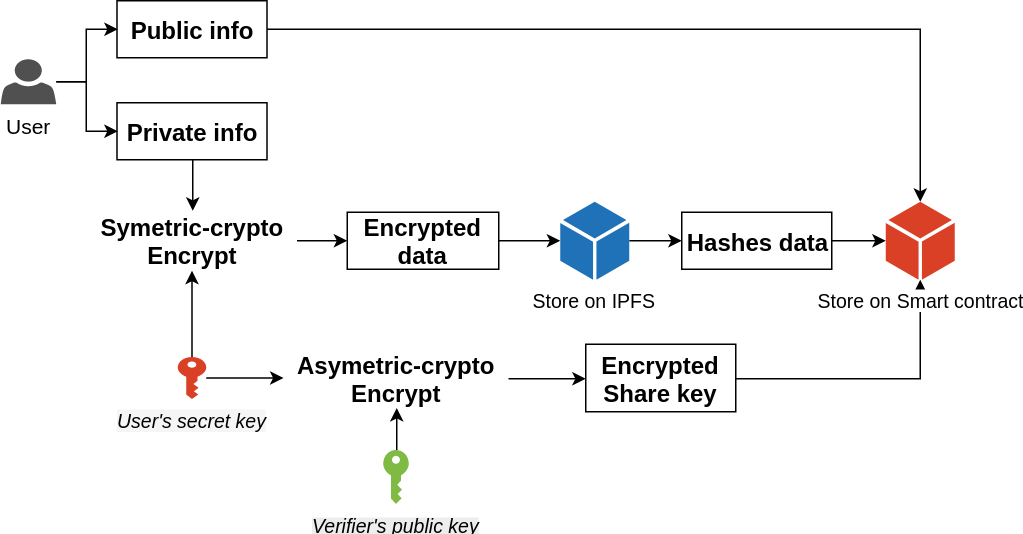
\includegraphics[scale=0.4]{identity-process-1}
\caption{Sơ đồ cách thức lưu trữ hồ sơ định danh}
\end{center}
\end{figure}

Việc chia sẻ hồ sơ định danh là quá trình chia sẻ các thông tin bí mật giữa verifier và người tạo lập hồ sơ phục vụ cho qui trình xác minh hồ sơ. Cách thức chia sẻ hồ sơ định danh được thể hiện trong hình \ref{fig:identity-process-2}:

\begin{itemize}
\item Verifier chọn một hồ sơ định danh của người dùng. Danh sách hồ sơ mà verifier duyệt là các hồ sơ mà người tạo hồ sơ đã chọn khóa công khai tương ứng với verifier đó.
\item Verifier sẽ nhập khóa bí mật (\textit{private key}) để giải mã \textit{SecretKey} của người dùng đã được mã hoá bởi khóa công khai của verifier trước đó.
\item Sau khi có được \textit{SecretKey} của người dùng, verifier sẽ tiến hành giải mã thông tin hồ sơ của người dùng.
\item Verifier dựa vào thông tin bí mật đã giải mã và tiến hành xác minh.
\end{itemize}

\begin{figure}[ht!]
\begin{center}
\label{fig:identity-process-2}
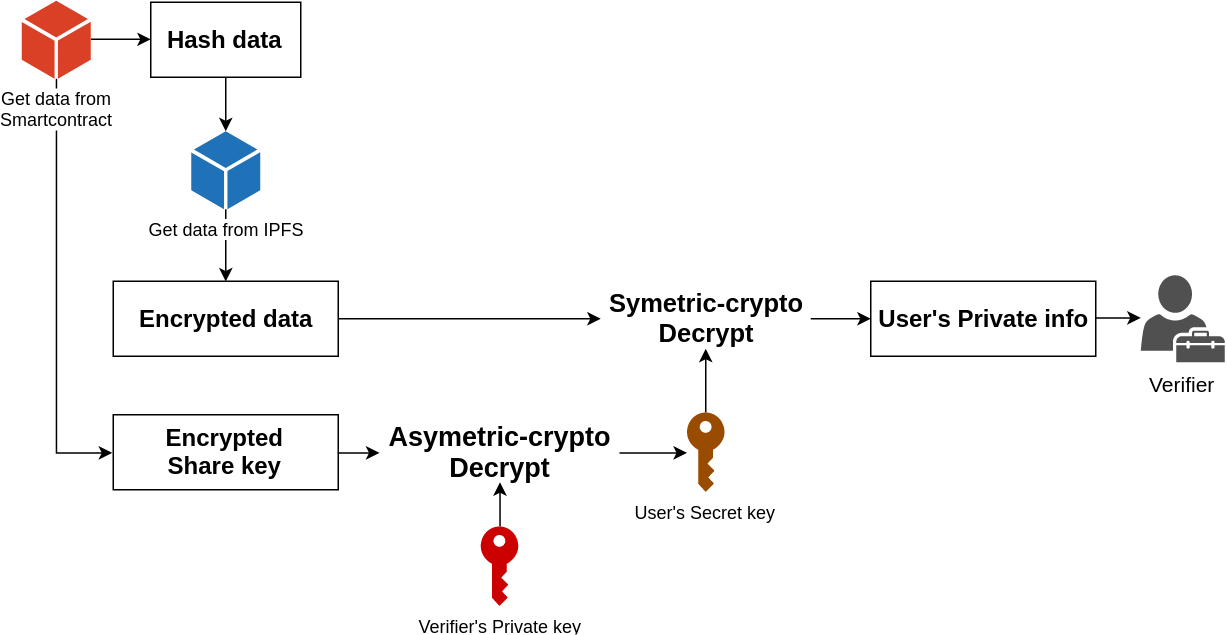
\includegraphics[scale=0.35]{identity-process-2}
\caption{Sơ đồ cách thức chia sẻ thông tin định danh}
\end{center}
\end{figure}

\subsection{Tạo lập và lưu trữ chiến dịch gây quỹ}
\subsubsection{Mục tiêu}

\subsubsection{Cách thức hoạt động}

\subsection{Chức năng giải ngân}
\subsubsection{Mục tiêu}
Việc giải ngân được thực hiện khi chiến dịch gây quỹ đạt được mục tiêu gây quỹ. Và giải ngân đối với chiến dịch sẽ được phân làm hai loại:

\begin{itemize}
\item \textbf{Giải ngân một giai đoạn} - sau khi chiến dịch gây quỹ hoàn thành mục tiêu gây quỹ trong thời gian đặt ra, thì người tạo chiến dịch có thể gọi lệnh giải ngân và rút được tiền từ chiến dịch.
\item \textbf{Giải ngân theo nhiều giai đoạn} - với một số chiến dịch có thể thực hiện theo nhiều giai đoạn khác nhau, thì việc giải ngân theo nhiều giai đoạn nhằm mục tiêu:
\begin{itemize}
\item Buộc người tạo chiến dịch có trách nhiệm báo cáo tiến độ thực hiện chiến dịch.
\item Tăng cường quyền của người đóng góp bằng cách bỏ phiếu đồng ý xác nhận giải ngân cho chiến dịch theo từng giai đoạn.
\end{itemize}
\end{itemize}

\subsubsection{Cách thức hoạt động}

\subsection{Hoàn tiền chiến dịch gây quỹ}
\subsubsection{Mục tiêu}

\subsubsection{Cách hoạt động}

\section{Tổ chức dữ liệu}
\subsection{Dữ liệu phi tập trung}

\subsection{Dữ liệu tập trung}

\end{document}